\section{Zielsetzung}
In diesem Versuch sollen Magnetfelder von verschiedener Spulenanordnung vermessen werden.
\section{Theorie}
Magnetische Felder werden erzeugt, wenn sich elektrische Ladung bewegt.
Dabei sind sie von Betrag und Richtung als Vektorgröße durch die magnetische Feldstärke
$\vec{H}$ beschrieben. Wichtig zu erwähnen ist das Magnetfelder kein Monopole besitzen
sondern immer paarweise auftreten und geschlossen sind im gegensatz zum elektrischen Monopol.
Die magnetische Flussdichte $\vec{B}$ wird über die Feldstärke $\vec{H}$ und über die
Permabilität $\mu$ zu der Formel:
\begin{equation}
  \vec{B} = \mu \cdot \vec{H}
  \label{eq:1}
\end{equation}
Dabei beschreibt die Permabilität $\mu$ die "Leitfähigkeit" des Materials und setzt sich
aus $\mu = \mu_0 \cdot \mu_r$ zusammen. $\mu_0$ ist die Vakuum-Permeabilität und beträg $4 \cdot \pi \cdot 10^{-7}$
und $\mu_r$ die relative Permeabilität der Materie.
Bei einem stromdurchflossenden Leiter verlaufen die Feldlinien in konzentrische Kreise und
stehen senkrecht zum Stromfluss. Mit Hilfe des Biot-Savartschen Gesetz lässt sich
das Magnetfeld mit einem Abstand $r$ und dem Strom $I$
\begin{equation*}
  d\vec{B} = \frac{\mu_0 I}{4\pi} \frac{d\vec{s} \times \vec{r}}{r^3}
\end{equation*}
berechnen. In Abbildung (\ref{abb:1}), folgt daraus für ein stromdurchflossene Spule die Formel:
\begin{equation}
  \vec{B}(x) = \frac{\mu_0 I}{2} \frac{R^2}{(R^2 + x^2)^{\frac{3}{2}}}
  \label{eq:2}
\end{equation}
\begin{figure}[H]
  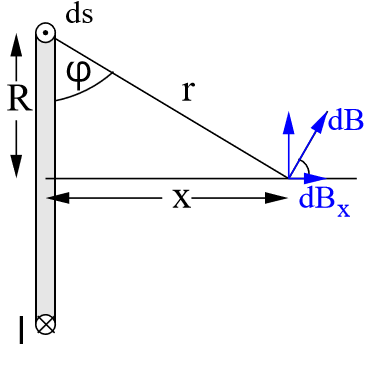
\includegraphics[width=5 cm , height=3.5 cm]{Abb1.png}
	\caption{Schematische Darstellung des Biot-Savartschen Gesetz[1].}
	\label{abb:1}
\end{figure}
Im Inneren für langgestreckten Spule (Solenoid) ist die magnetische Feldstärke $\vec{H}$
homogen und konstant während es ausserhalb inhomogen ist.
Mit der Spulenlängen $l$, der Windungszahl $n$ und dem Strom $I$ lässt sich das
homogene Magnetfeld mit der Formel
\begin{equation}
  B = \mu_r \mu_0 \frac{n}{l} I
  \label{eq:3}
\end{equation}
darstellen. Wird die langgestreckte Spule zu einem Kreis gebogen so wird die Spulenanordnung
als Torus bezeichnet. Die Besonderheit des Torus ist, dass ausserhalb kein Magnetfeld
existiert und im Inneren das Magnetfeld homogen. Somit lässt sich die Gleichung(\ref{eq:3})
mit $l= 2\pi r_T$ zu
\begin{equation}
  B = \mu_r \mu_0 \frac{n}{2\pi r_T} I
  \label{eq:4}
\end{equation}
umschreiben. Dabei ist $r_T$ der Radius des Torus.
Ein andere Verfahren zu Herrichtung eines homogen Magnetfeldes ist die Helmholz-Spule.
Zwei parallele Kreisspulen, die die gleiche Stromrichtung besitzen, erzeugen ein homogens
Feld im Inneren der beiden Spulen. Eine Darstellung ist in Abbildung(\ref{abb:2}) zu sehen.
\begin{figure}[H]
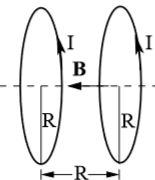
\includegraphics[width =10 cm, height = 7cm]{Abb2.png}
\caption{Schematische Darstellung der Helmholz-Spule[1].}
\label{abb:2}
\end{figure}
Mit Hilfe der Gleichung (\ref{eq:2}) lässt sich das Magnetfeld
\begin{equation}
  B(0)=B_1(x_1) + B_1(-x_1) = \mu_0 I \frac{R^2}{(R^2 + x^2)^{\frac{3}{2}}}
  \label{eq:5}
\end{equation}
beschreiben. Dabei ist $x=\frac{d}{2}$ mit $d$ als Abstand der beiden Spulen.
